%%%%%%%%%%%%%%%%%%%%%%%%%%%%%%%%%%%%%%%%%%%%%%%%%%%%%%%%%%%%%%%%%%%%%%%%%%%%%%%%%%%%%%%%%%%%%%%%%%%%%%
%
%   Filename    : chapter_3.tex 
%
%   Description : This file will contain your Research Methodology.
%                 
%%%%%%%%%%%%%%%%%%%%%%%%%%%%%%%%%%%%%%%%%%%%%%%%%%%%%%%%%%%%%%%%%%%%%%%%%%%%%%%%%%%%%%%%%%%%%%%%%%%%%%

\chapter{Theoretical Framework}
\begin{comment}
This chapter lists and discusses the specific steps and activities that will be performed by the proponent to accomplish the project. 
The discussion covers the activities from pre-proposal to Final Thesis Writing.  It also includes an initial discussion on the theoretical framework to be followed.
Research activities include inquiry, survey, research, brainstorming, canvassing, consultation, review, interview, observe, experiment, design, test, document, etc.  
The methodology also includes the following information:
\begin{itemize}
   \item who is responsible for the task
   \item the resource person to be contacted
   \item what will be done
   \item when and how long will the activity be done
   \item where will it be done
   \item why should be activity be done
\end{itemize}
\end{comment}

\begin{figure}[b]
   \centering                    
   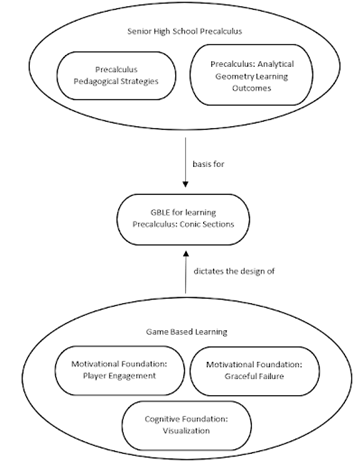
\includegraphics{theoreticalframework.png}
   \caption{Theoretical Framework}
    \label{fig:theoreticalframework}
\end{figure}

In this chapter, a theoretical framework consisting of a Game Based Learning Environment (GBLE) is used as a learning tool for precalculus pedagogy. The design of the GBLE is dictated based on three foundations, particularly player engagement,graceful failure, and visualization. The proposed GBLE uses Senior High School Precalculus Pedagogical Strategies and Analytical Geometry Learning Outcomes as a backbone for targeting Conic Sections. There are several sections below to further discuss each component of the theoretical framework in more detail.

\section{Game Based Learning}
There are three foundations under the game based learning section which will be the backbone of the GBLE to be created. Specifically, these are player engagement, graceful failure, and visualization. Each of these elements are to be discussed in further detail in every subsection below.

\subsection{Motivational: Player Engagement}
According to Schoenau-Fog (2011), the engagement must be sustained in order to motivate a player to keep playing, this means that good games must be engaging enough so players would want to keep playing them. Sharek (2018) states that engagement is the willingness of a person to participate in something, and that it cannot stand alone if they are cognitively underloaded. The GBLE to be created seeks to balance the amount of cognitive engagement of the players so they will continue to want to be engaged in the game. This could be done in several ways such as giving the players challenges that are not easily attainable but at the same time achievable. Gregory, E. (2008) made use of The Experience Sampling Method (ESM) to investigate how people feel, think, and do in their lives. This information was then used to create stories that are used in video games, and these stories help in making players more engaged as the stories were based on the feelings of people that define their experience of wanting to become more engaged in tasks. With all of these elements combined as the backbone for creating GBLEs, players would become more engaged in the game, and this can increase the ability of GBLEs to be used in an educational setting.

\begin{figure}[t]
   \centering                    
   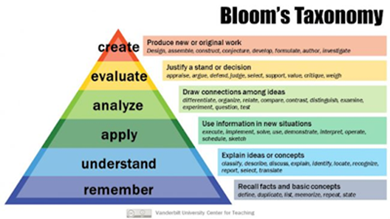
\includegraphics{bloomtaxonomy.png}
   \caption{Bloom's Taxonomy}
    \label{fig:bloomtaxonomy}
\end{figure}

According to the framework of Bloom’s Revised Taxonomy (2001), in order to assess how to develop proper learning outcomes, a hierarchy was created in order to differentiate levels of how much cognitive learning do students experience. At the top of this framework we’re the three most effective ways of cognitive learning, namely: create, evaluate, analyze. By focusing on these methods, the proposed GBLE offers learners the highest form of cognitive learning experience possible.

\subsection{Motivational Foundation: Graceful Failure}
Litts, B., \& Ramirez, D. (2014) argue that the deepest learning occurs when one fails. As failing provides an opportunity to learn from failure and further saying that learning is an iterative process of incomplete constructs and revisions which is propelled by failure. GBLEs are able to provide spaces where the consequences of failure are low, encouraging learners to take risks and try new strategies to reach their goals at their own self-regulated pace (Plass et al., 2015).

\subsection{Cognitive Foundation: Visualization}
According to Hazzard (2015), data visualization augments cognition and has different purposes such as a health bar to display a character’s status, or a skill tree showing the potential of a character. Hazzard divided data visualization used in games into two primary types: status information and training. Status information allows players to have planned choices, give players information, or both. Zammitto (2008) states that video games rely on the information players see on the screen, so if the information is not correctly visualized, it can lead to a frustrating experience for the players. Zammitto also states that a good interface is one that is not noticed. These can be included when creating GBLEs as it will be able to support the decisions that players make depending on the information they can visualize. This is especially important when GBLEs are to be used as an educational tool, as the information displayed will be very crucial in helping the players learn what the game intends for them to learn.

\section{Senior High School Precalculus}
This section contains the learning outcomes and pedagogies that will be the basis for creating a GBLE for learning Precalculus: Conic Sections. The Learning Outcomes are expected to be learned by the student players as they interact with the proposed GBLE, and the pedagogical strategies are to be used in order to have a guide in teaching Precalculus: Conic Sections through a GBLE.

\subsection{Precalculus Pedagogical Strategies}
The GBLE to be created seeks to include the strategies provided by DepEd as these pedagogies have already been used, and the efficient strategies can be used as a guide for implementing ways on how the GBLE can be used as an educational tool in helping Senior High School students learn Precalculus better. Due to DepEd's protocol for teachers to give them academic freedom to teach the way they deem appropriate for learners, there's a variety of strategies available for each individual student. But since the problem is mostly in foundation skills, most of the strategies include review of these foundational skills as well as applying such knowledge to real life situations.
\subsection{Precalculus: Analytical Geometry Learning Outcomes}
Based on the curriculum guide of DepEd for Grade 11 STEM Pre-Calculus, two LOs were chosen from the contents of Analytic Geometry through the recommendation of a Precalculus expert. The target LOs were Learning Competency 14 and 15. The first LO expects the learners to recognize the equation and important characteristics of the different types of conic sections, while the second LO expects them to solve examples of real life problems involving conic sections. To assist the player-learners in mastering these LOs would be the primary objective of the proposed GBLE for Precalculus. Both of these LOs can be targeted by a single game mechanic in the GBLE in which the players would be asked to solve puzzles in the game depicting real-world situations where the concept of Conic Sections were being applied. These puzzles would be supported with the context provided by the game’s story narration.

\section{GBLE for Learning Precalculus: Conic Sections}
The proposed GBLE for learning Precalculus Conic Sections will be using the concepts mentioned within the theoretical framework of the study. The target LOs for the Conic Sections would be the basis for how each of the GBLE’s mechanics, designs, and scenarios will be made in order for the learners to understand the concepts within the topic of Conic Sections. For example, certain learning game design principles will be followed to provide appropriate game mechanics to target the appropriate LOs by simulating real-world situations in the game where the concepts of Conic Sections should be used in order to make progress within the game. The GBLE’s goal is to provide a way for the students to learn more about the topic in a more engaging way as compared to the traditional classroom method.

